

%\begin{figure}[ht]
%\centering
%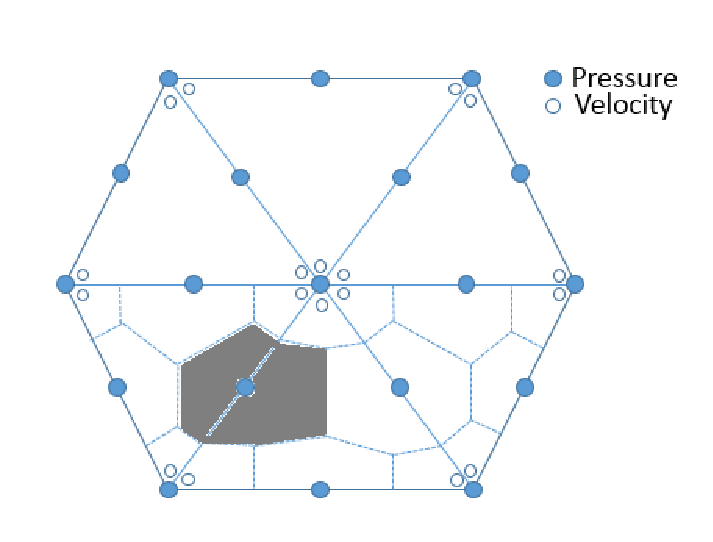
\includegraphics[width=.5\textwidth]{./Pics/P1DGP2.pdf}
%\caption{2D representation of the $P_{1}DGP_{2}$ element pairs used in this work. Shaded areas denote control volumes (in which saturation field is stored)blue points represent the pressure nodes and white points the velocity nodes.}
%\label{fig:fem_cv}
%\end{figure}

%\begin{figure}[ht]
%   \vbox{
%       \hbox{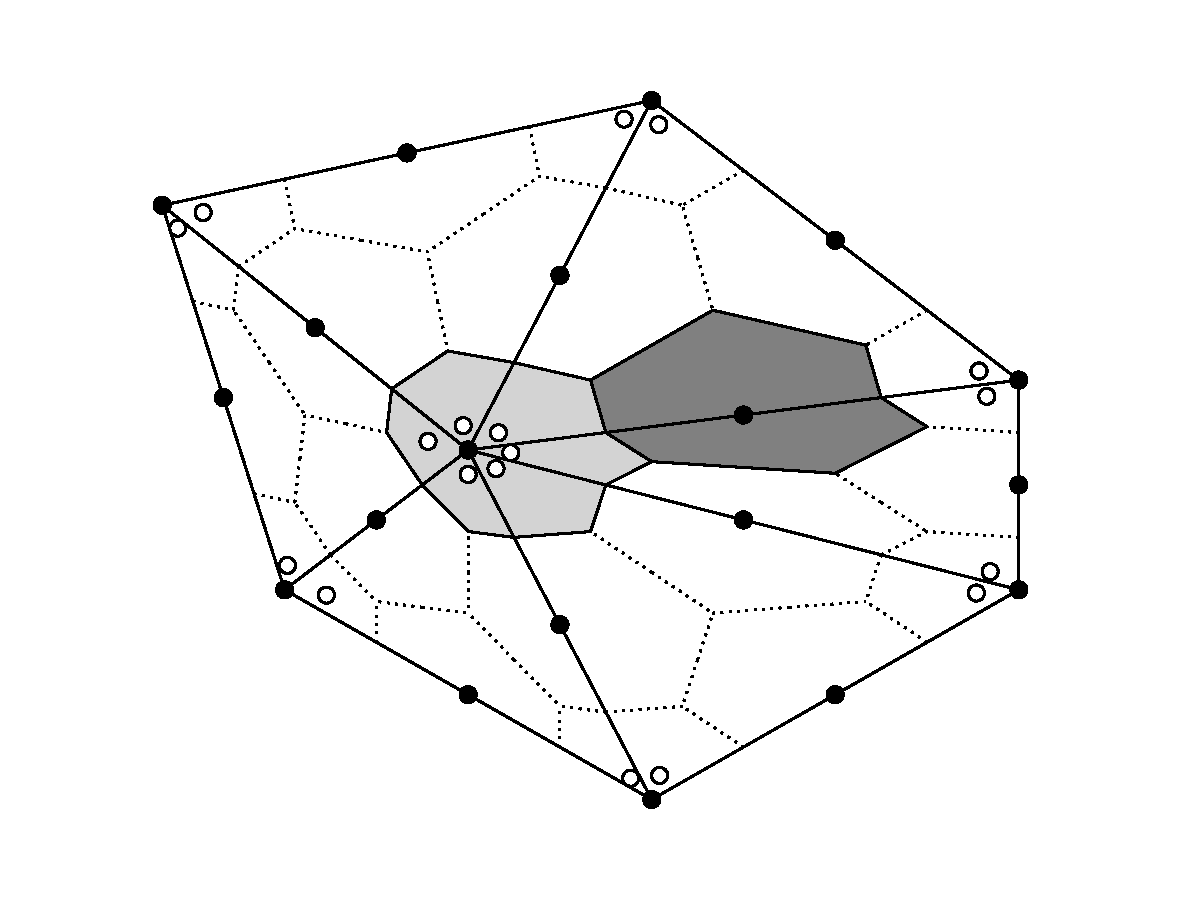
\includegraphics[width=.5\textwidth]{./Figs/p1dgp2-cont-sat.pdf}
%             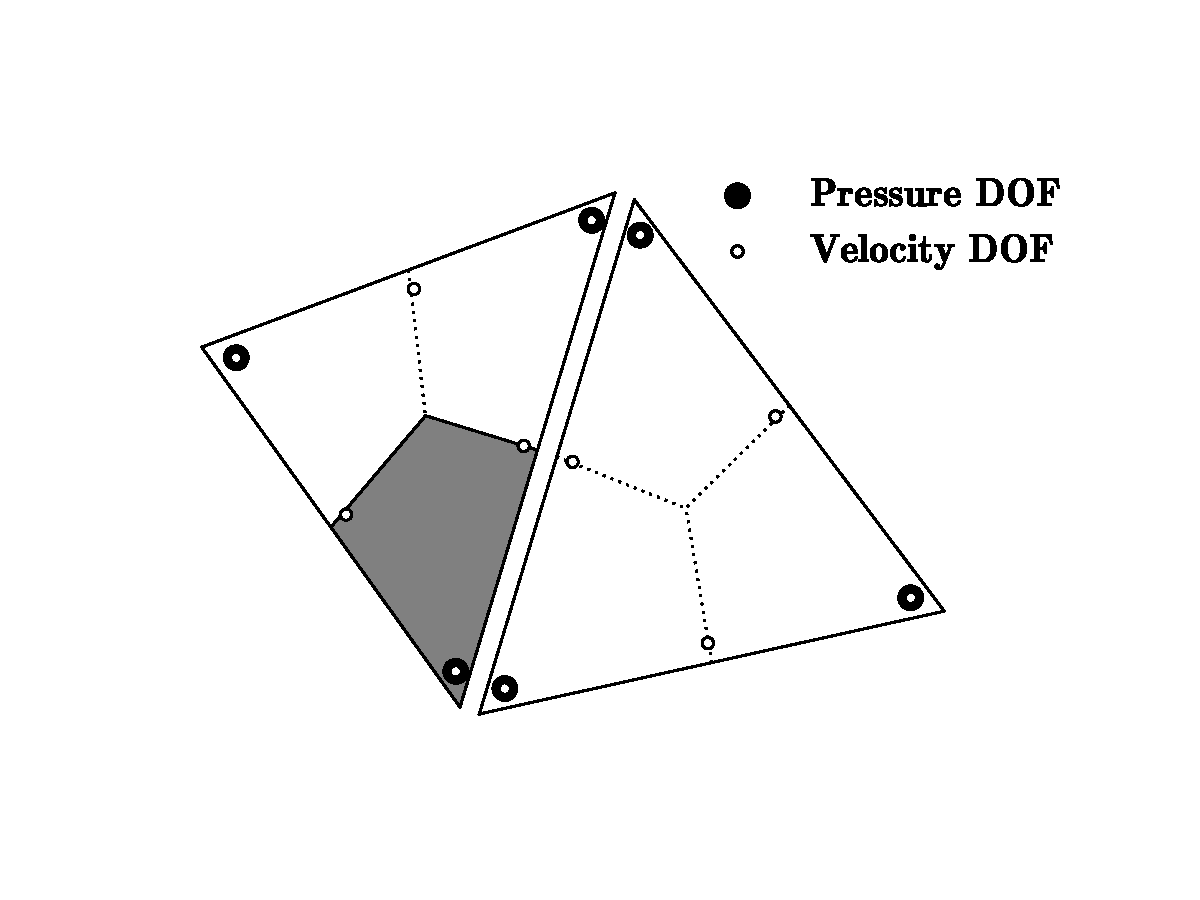
\includegraphics[width=.5\textwidth]{./Figs/p2dgp1-dg-sat.pdf}}
%       \hbox{\hspace{3cm}(a) \PN[1]{2} \hspace{5.cm} (b)\PNDG[2]{1}}}
%\caption{2D representation of the element pairs presented in this work. Shaded areas denote control volumes (in which saturation is   stored), black points represent the pressure nodes and white points the velocity nodes. Note that in (b) velocity and pressure nodes overlap in the triangles' vertices.}
%    \label{fem_cv_represent_a}
%\end{figure}


%%%%
%%%%  FIGURE 1
%%%%
\begin{figure}[ht]
\centering
\vbox{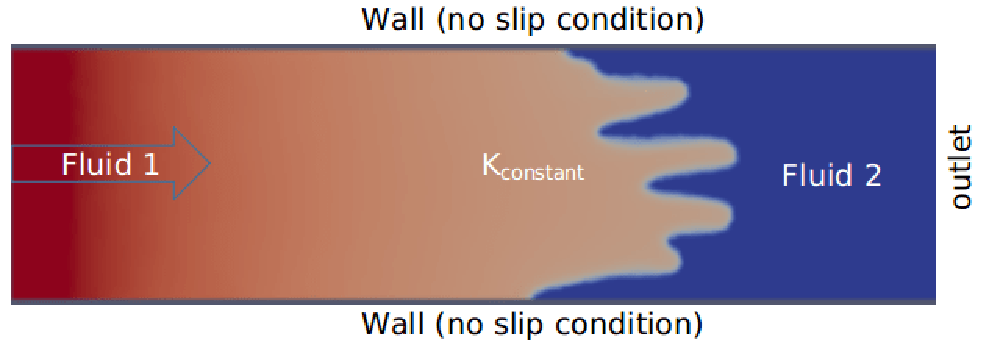
\includegraphics[width=\textwidth]{./Pics/phase_vol_frac_uni_perm_1}}
\caption{Schematics of flow instabilities during injection of a pure low viscosity fluid (left-hand side in red) into a domain saturated with a second fluid (dark blue). The ratio of viscosity between the two fluids is 5. In this case, the initially piston shape front collapses leading to the formation of several fingers.}
\label{fig:simple_case}
\end{figure}
\clearpage



%%%%
%%%%  FIGURE 2
%%%%
\begin{figure}[ht] 
\vbox{
\hbox{\hspace{1cm}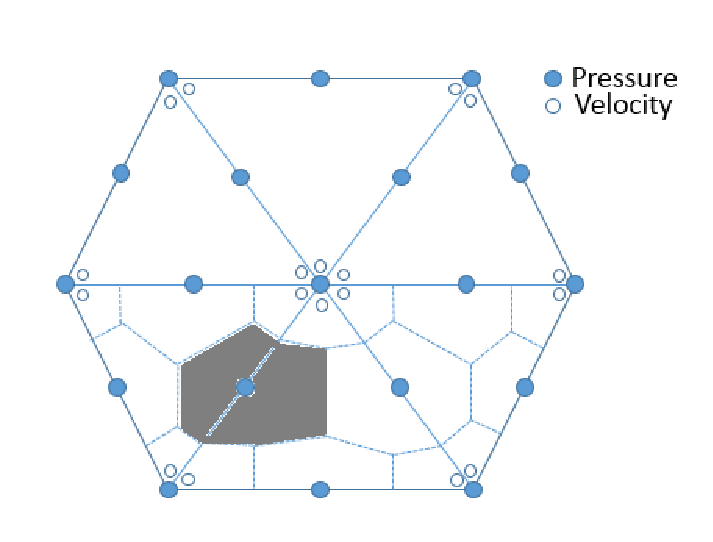
\includegraphics[width=.7\textwidth]{./Pics/P1DGP2}}
\hbox{\hspace{6cm}(a)}
\vspace{.5cm}
\hbox{\hspace{1cm}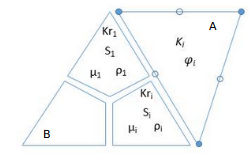
\includegraphics[width=.7\textwidth]{./Pics/element_n}}
\hbox{\hspace{6cm}(b)}}
\caption{Sketches of FE-pairs: (a) 2D representation of the \PN[1]{2} element-pair used in this work. Shaded areas denote control volumes (in which scalar fields such as phase saturation, temperature, density etc are stored); blue and white circles represent pressure and velocity nodes, respectively. (b) Simplified representation of field storage in a \PN[1]{1} element-pair: permeability $\left(K_{i}\right)$ and porosity $\left(\phi_{i}\right)$ are stored in $P_{0}DG$ space ($A$), whereas all other scalar fields (e.g., saturation, density, viscosity, relative permeability etc) are stored in CV space ($B$). \red{(KOSTAS, COULD YOU: (a) REPLACE 1 BY i (top quad of ELEMENT B) AND (b) REMOVE THE WHITE CIRCLES IN ELEMENT A)}.}
\label{fig:fem_cv}
\end{figure}

